\chapter{Implementation}\label{chapter:implementation}
\section{Plugin}
iBSched is implemented as an extension to SLURM in the form of a scheduler plugin. A Slurm plugin is a dynamically linked code object which is loaded explicitly at run time by the Slurm libraries. A plugin provides a customized implementation of a well-defined API connected to tasks such as authentication, interconnect fabric, and task scheduling. There are several other existing scheduler plugins of SLURM such as: the default(FCFS) plugin, Backfill, wiki and wiki2(Interfaces to external schedulers) etc. A related plugin that is of importance to scheduling is the priority plugin because the job queue is first constructed and then sorted based on priorities before the scheduling algorithm runs through it. Slurm provides a basic priroity plugin and a multifactor priority plugin. The basic version provides a standard FIFO based job priority whereas the multifactor version provides priorities to job based on several factors such as age, fair-share, job size(also considers the job duration to calculate a weight factor for job size relative to time), partition, quality of service etc. The multifactor priority plugin has been refactored for this work to be better suitable for our implementation. Specifically, the multifactor priority plugin now assigns priority to jobs based on age and size(relative to time). As its default behavior it periodically re-calculates the priorities of the jobs.\\ \\
%%%%%
For the current scope of the work, iRTSched has been implemented as an independent binary that talks to iBSched via the negotiation protocol. The purpose of this independent binary is to fake an actual runtime scheduler by simulating the runtime states of the system in time by employing the runtime scheduling algorithm and also negotiating with iBSched. In reality, a full-fledged runtime scheduler will be managing the resources in the invasic partition, will launch the jobs and perform dynamic resource management. In order to evaluate the negotiation-based separation of batch and runtime scheduling system, a simulation of the same would be very useful and sufficient for our objectives. 
\section{Data Structures}
This section will enumerate some of the important data structures that are a part of the implementation.\\ \\
\lstset{breaklines=true}
\textbf{Job Mappings}\\
Below is enum that represents the possible characterstics of a job. This hint can be supplied at job submission time or can be inferred during runtime and profiling the application performance. By default it will be considered as NONE.
\begin{lstlisting}[mathescape]
enum job_hint {
        COMP_BOUND,
        MEMORY_BOUND,
        IO_BOUND,
	NONE
};
\end{lstlisting}
Below is an enum that represents the type of a job. This needs to be specified at submission time by the user. By default it will be considered as rigid.
\begin{lstlisting}[mathescape]
enum job_type {
        RIGID,
        MOLDABLE,
        EVOLVING,
        MALLEABLE
};
\end{lstlisting}
Below structure represents the node count constraint that is used by the batch scheduler during the negotiations with runtime scheduler. At the submission time max will be set to the job's max nodes and min will be set to a value of max nodes - step\_size where step\_size is calculated from the formula given in x.x. This step will be repeated when a new transaction starts.
\begin{lstlisting}[mathescape]
typedef struct qos_rsrc {   
        uint32_t min;
        uint32_t max;
} qos_rsrc_t;
\end{lstlisting}
%%%%%%%%
Below structure represents the details of a job necessary for its launch. This is packed within the following structure and it gets forwarded to the runtime scheduler.
\begin{lstlisting}[mathescape]
struct forward_job_details {
        qos_rsrc_t node_count;          /* Job resource requirements */
        uint16_t cpus_per_task;         /* number of processors required for
                                         * each task */
        uint8_t hint;                   /* Job characteristic: IO / Compute / Memory bound */
        uint8_t job_type;                       /* Type of job: Static or Dynamic */
        /* Ideally this structure should further contain all the necessary details required for launching this job. For the purpose of this thesis, we are only doing a simulation without running jobs, hence other details in this structure are not important */
};
\end{lstlisting}
%%%%%%%
The below structure makes up a single entry in the Map that is constructed by batch scheduler. A list of such entries make up the mapping of jobs to offer which is sent to the runtime scheduler. In addition to the details of the job as mentioned for the previous structure, this structure include details such as the bitmap of nodes allocated, priority, job id, min / max nodes etc.
\begin{lstlisting}[mathescape]
struct forward_job_record {
        struct forward_job_details *details;    /* job details */
        uint32_t job_id;                /* job ID */
        uint32_t magic;                 /* magic cookie for data integrity */
        char *name;                     /* name of the job */
        bitstr_t *node_bitmap;          /* bitmap of nodes allocated to job */
        uint32_t node_cnt;              /* Current node count assigned */
        uint32_t min_nodes;
        uint32_t max_nodes;
        uint32_t priority;              /* relative priority of the job,
                                         * zero == held (don't initiate) */
        time_t start_time;              /* Expected or Actual start time */
        uint32_t time_limit;            /* time_limit minutes or INFINITE,
                                         * NO_VAL implies partition max_time */
        uint32_t time_min;              /* minimum time_limit minutes or
                                         * INFINITE,
                                         * zero implies same as time_limit */
};
\end{lstlisting}
%%%%%%%
Below structure represents the message used by batch scheduler to request for a resource offer. It contains a value field used for the purpose of protocol communication followed by the most important field which is the Map.
\begin{lstlisting}[mathescape]
typedef struct request_resource_offer_msg {
        uint16_t value; /* info */
        List jobs2map; /* This is the list of jobs waiting to be dispatched. And communicates the current requirements to rt scheduler which 
                          can then try to suitably construct a resource offer to satisfy the requirements as best as possible */
} request_resource_offer_msg_t;
\end{lstlisting}
%%%%%%%%
Below structure represents the response to a resource offer sent by the batch scheduler. It resembles very closely to the previous message but has in addition the error code and the error msg fields. These fields which identify the error are important for batch scheduler to convey its response to the runtime scheduler for the offer it sent.
\begin{lstlisting}[mathescape]
typedef struct resource_offer_resp_msg {
        uint16_t value;         /* info */
        List map_jobs2offer;    /* Jobs mapped to the given offer. This depends on whether the batch scheduler accepted / rejected / countered
                                 the resource offer it received */
        uint32_t error_code;    /* error code on failure */
        char   * error_msg;     /* error message on failure */
} resource_offer_resp_msg_t;
\end{lstlisting}
%%%%%%%
\textbf{Resource Offers}\\
Below structure represents the reservation for a job which can begin immediately or in the future. This depends on the response from the runtime scheduler.
\begin{lstlisting}[mathescape]
typedef struct job_resv {
        time_t end_time;        /* end time of reservation              */
        uint8_t full_nodes;        /* when reservation uses full nodes or not */
        uint32_t job_id;        /* job ID */
        bitstr_t *node_bitmap;  /* bitmap of reserved nodes             */
        uint32_t node_cnt;      /* count of nodes required              */
        time_t start_time;      /* start time of reservation            */
} job_resv_t;
\end{lstlisting}
Below structure represents the message format for resource offer message sent by runtime scheduler. It contains a list of reservations for each of the jobs that were sent by batch scheduler in its mapping. It contains the set of residual or free nodes available.
\begin{lstlisting}[mathescape]
typedef struct resource_offer_msg {
        uint16_t value;      /* info */
        uint8_t negotiation; /* if negotiation is ongoing then this value is 1 else it becomes 0 to indicate ischeduler that previous negotiat
                                ion is over */
        List resource_offer;   /* List of node space records */
        List resv_jobs;        /* List of jobs with actual reservations. Can also include jobs with virtual reservations that are those with
                                  future start / service times */
        uint32_t error_code;    /* error code on failure */
        char   * error_msg;     /* error message on failure */
} resource_offer_msg_t;
\end{lstlisting}
%%%%%%%%%%
\textbf{Feedback Reports}\\
Below structures represent the format of a feedback report and a list of reports respectively. For the scope of this current work, the feedback does not send back any performance model of the running / completed application or any kind of job characteristic and energy consumption. It sends across basic details about the status of running / completed jobs.
\begin{lstlisting}[mathescape]
typedef struct job_status {
        uint32_t job_id;
        time_t run_time;
        time_t end_time;
        uint32_t node_cnt;
        bitstr_t *node_bitmap;
        uint32_t job_state;
} job_status_t;

typedef struct status_report_msg {
        List status_reports;
} status_report_msg_t;
\end{lstlisting}
%%%%%%%%%%%
\textbf{Running Job Record}\\
The below structure is very important as the runtime scheduler uses this as the job record for each of the running jobs. Since the scope of this work is simulation, We do not include many other details of a job that would be necessary for its launch, logging etc. Dependency of a forwarded job onto a running malleable job is saved in the variables depend\_job\_id and depend\_job\_prio of a running job record. This dependency information is used by the PDBES algorithm.
\begin{lstlisting}[mathescape]
struct run_job_record {
        uint32_t job_id;
        bitstr_t *node_bitmap;
        time_t start_time;
        uint32_t priority;
        uint32_t time_limit;
        uint8_t hint;
        uint8_t job_type;
        time_t end_time;
        time_t orig_end_time;
        uint32_t job_state;
        uint32_t orig_node_cnt;
        uint32_t node_cnt;
        uint32_t last_node_cnts[2];
        bitstr_t *next_node_bitmap;
        uint32_t next_node_cnt;
        uint32_t depend_job_id;
        uint32_t depend_job_prio;
        uint32_t save_depend_job_id;
        uint32_t save_depend_job_prio;
        uint32_t min_nodes;
        uint32_t max_nodes;
        uint8_t adapt;  /* 0 - No change, 1 - Expand, 2 - Shrink */
        uint8_t transformed;
        time_t exp_end_time;
};
\end{lstlisting}
%%%%%%%
\textbf{Node Space Map}\\
Below is an existing structure used by SLURM for its backfilling algorithm. This is used to form a chain of records chronologically ordered in time that represent the set of available nodes in those timeslots. The backfill algorithm uses this structure to prepare the view of resources in time and resembles a two dimensional space of nodes and time. This is used in order to compute when and where a job can start by looking at the reservations that higher priority jobs already have and these must be respected by lower priority jobs in case they can start now.
\begin{lstlisting}[mathescape]
typedef struct node_space_map {
        time_t begin_time;
        time_t end_time;
        bitstr_t *avail_bitmap;
        int next;       /* next record, by time, zero termination */
} node_space_map_t;
\end{lstlisting}
%%%%%%%%
\section{Important APIs}
\begin{lstlisting}[mathescape,frame=single]
extern List schedule_invasic_jobs(resource_offer_msg_t *, List, uint16_t *, uint32_t *);
\end{lstlisting}
This routine is responsible for creating a map of jobs to the available offer. It will fill the offer that has been passed as a an argument to it with the list of invasive jobs that have been selected according to its algorithm. Jobs in this list would be mapped to some number of nodes that satisfy the job constraints. Those jobs which could not be mapped will have their constraints relaxed and just forwarded along with other jobs. Also, The batch scheduler has a limit on the number of jobs that can be forwarded but have not been mapped to any resources as it did not satisfy its constraints. This is the reservation depth similar to what is used in backfill algorithms. Once the limit has been reached the scheduling algorithm will then just scan the rest of the invasive job queue to look for jobs that can fit the remaining available nodes in the offer.\\ 
\begin{lstlisting}[mathescape,frame=single]
extern uint32_t adjustQoS_node_count(struct job_record *);
\end{lstlisting}
This routine relaxes the node count constraint of a job. The original constraints are min and max nodes supplied at the job submission time. Negotiation begins by setting a node count constraint(node\_count.min, node\_count.max) within this window of min and max. With more negotiation attempts in a single transaction, the constraints would keep getting relaxed and node\_count.min would approach the original min value.\\
\begin{lstlisting}[mathescape,frame=single]
extern void resetQoS_node_counts();
\end{lstlisting}
This routine is called before the start of a new set of negotiations. It will reset the node count constraint for every job in the queue to their original values.\\
\begin{lstlisting}[mathescape,frame=single]
extern int _decision_logic(List, int, uint32_t);
\end{lstlisting}
This routine is where the batch scheduler makes a final decision on whether the received resource offer form runtime scheduler is accepted / rejected. It does so by checking through the mapping that has been constructed after the scheduling algorithm processed the offer. The mapping is supplied as the first argument to this function.\\
\begin{lstlisting}[mathescape,frame=single]
extern void *irm_agent(void *);
\end{lstlisting}
This is the routine that is associated with the main runtime scheduler thread. It gets called once the thread has been created. It basically runs an infinite control loop for the scheduler to initiate various operations such as processing the response for an offer from batch scheduler, performing a transformation of the runtime system state, waiting for a request for resource offer in a separate spawned thread, sending back an offer to batch scheduler, terminating the scheduler etc.\\
\begin{lstlisting}[mathescape,frame=single]
extern int process_resource_offer(resource_offer_msg_t *, uint16_t *, int *, List *, List);
\end{lstlisting}
This routine initiates the processing of a resource offer, calls the appropriate scheduling algorithm.\\
\begin{lstlisting}[mathescape,frame=single]
extern int _request_resource_offer(slurm_fd_t);  /* Wrapper for request_resource_offer to construct the list of job requirements to be sent */
\end{lstlisting}
This routine sends a request for resource offer to the runtime scheduler. It does so by constructing a list of job requests to be forwarded.\\
%%%%%%%%%%%%%
\begin{lstlisting}[mathescape,frame=single]
extern int process_rsrc_offer_resp(resource_offer_resp_msg_t *, int, resource_offer_msg_t **);
\end{lstlisting}
This routine is responsible for processing the mapping received from the batch scheduler and invoking the appropriate runtime scheduling algorithm. If the response from batch scheduler was accept for its previous offer, then it will recreate the transformation of the previous attempt else it will create a new transformation. It will run the algorithm to satisfy as many jobs forwarded as possible by using the PDBES algorithm and then determine whether it will accept / reject this mapping. If it does not accept then it will send a new offer created as a result of this new transformation.\\
\begin{lstlisting}[mathescape,frame=single]
extern int create_resource_offer(int, List, uint16_t, resource_offer_msg_t **);
\end{lstlisting}
This routine is called from within the "process\_rsrc\_offer\_resp" routine to initiate the scheduling algorithm to run through the mapping. It is also called in the "irm\_agent" routine in situations when a request for a resource offer is received. Or, a new offer needs to be generated by the runtime scheduler since some running applications have shrunk to create a gap in the resources that can be utilized to serve some new batch jobs.\\
\begin{lstlisting}[mathescape,frame=single]
static int 
_schedule(int attempts, List job_queue,
                uint16_t *recv_err_code, resource_offer_msg_t **rsrc_offer_msg);
\end{lstlisting}
This is the runtime scheduling algorithm whose steps have been described in the form of a pseudo code x.x.x. It will use the PDBES algorithm to scan through the mapping and provide start times for each of them.\\
\begin{lstlisting}[mathescape,frame=single]
extern bitstr_t * _try_transf(bool);
\end{lstlisting}
This routine performs a runtime transformation of the system state by performing expand / shrink of the running malleable jobs considering their performance and scalability. In case the result of this transformation are some free resources, then those will be sent up to batch scheduler as a new resoruce offer. The boolean argument passed here represents the negotiation flag. If it is true then it means we have received a request for an offer and must perform a partial transformation by doing only the shrink operations to create a gap in the resources. If it is false then it means that we must do the full transformation as no offer is being sent out.\\
\begin{lstlisting}[mathescape,frame=single]
extern int _commit_state(bool);
\end{lstlisting}
This routine will commit the forwarded jobs(with immediate start time) to the running jobs list. It will also change the node bitmaps of running jobs to their new node bitmaps if they have been subjected to some sort of transformation during the phase of runtime scheduling algorithm. In alignment with the new node counts for many of the running malleable jobs, there expected end times will also be updated based on whatever performance model is know until this point.\\
\begin{lstlisting}[mathescape,frame=single]
extern bool _get_delta(uint32_t *, time_t, time_t);
\end{lstlisting}
This routine will compute the next time slice for which the runtime scheduler will sleep. This could be a fixed time interval for periodic wake ups of the runtime scheduler or it can wake up earlier if there was some job that is expected to complete within this time interval.
\begin{lstlisting}[mathescape,frame=single]
extern void _initialize_state(void);
\end{lstlisting}
This routine resets the state of the system back to the point before the start of the negotiation. During the negotiation process, a lot of the details in the running job records would be temporarily updated to account for negotiations and the associated expand / shrink operations. With every negotiation attempt within a transaction, the state will have to be reset before the runtime scheduler can run its algorithm again.\\
\begin{lstlisting}[mathescape,frame=single]
extern int _decision_logic(resource_offer_msg_t *, List, int, bool);
\end{lstlisting}
The runtime scheduler decides whether to accept / reject the mapping received from batch scheduler by calling this routine. This routine checks through the mapping to see how many jobs can be started immediately and based on how well it is suitable for its metrics a decision will be taken.
%%%%%%%%%%%%%
\section{State Machine Diagrams}
Following pages give the state machines diagrams of both the batch and the runtime scheduler. These diagrams illustrate their implementation and the general flow of their working highlighting the important details. Many of the error handling or subordinate threads related to feedback, urgent job handling, signal handling for termination etc. have not been shown here due to space constraints. The diagrams in both the pages represent the main control thread for both the batch and runtime scheduler. This control thread is responsible to spawn other subordinate threads, drive the control loop responsible for doing / initiating all the work such as receiving processing and sending protocol messages.\\ \\
%%%%%%%%
\begin{figure}[!htbp]
\hspace*{0.1in}
\centering
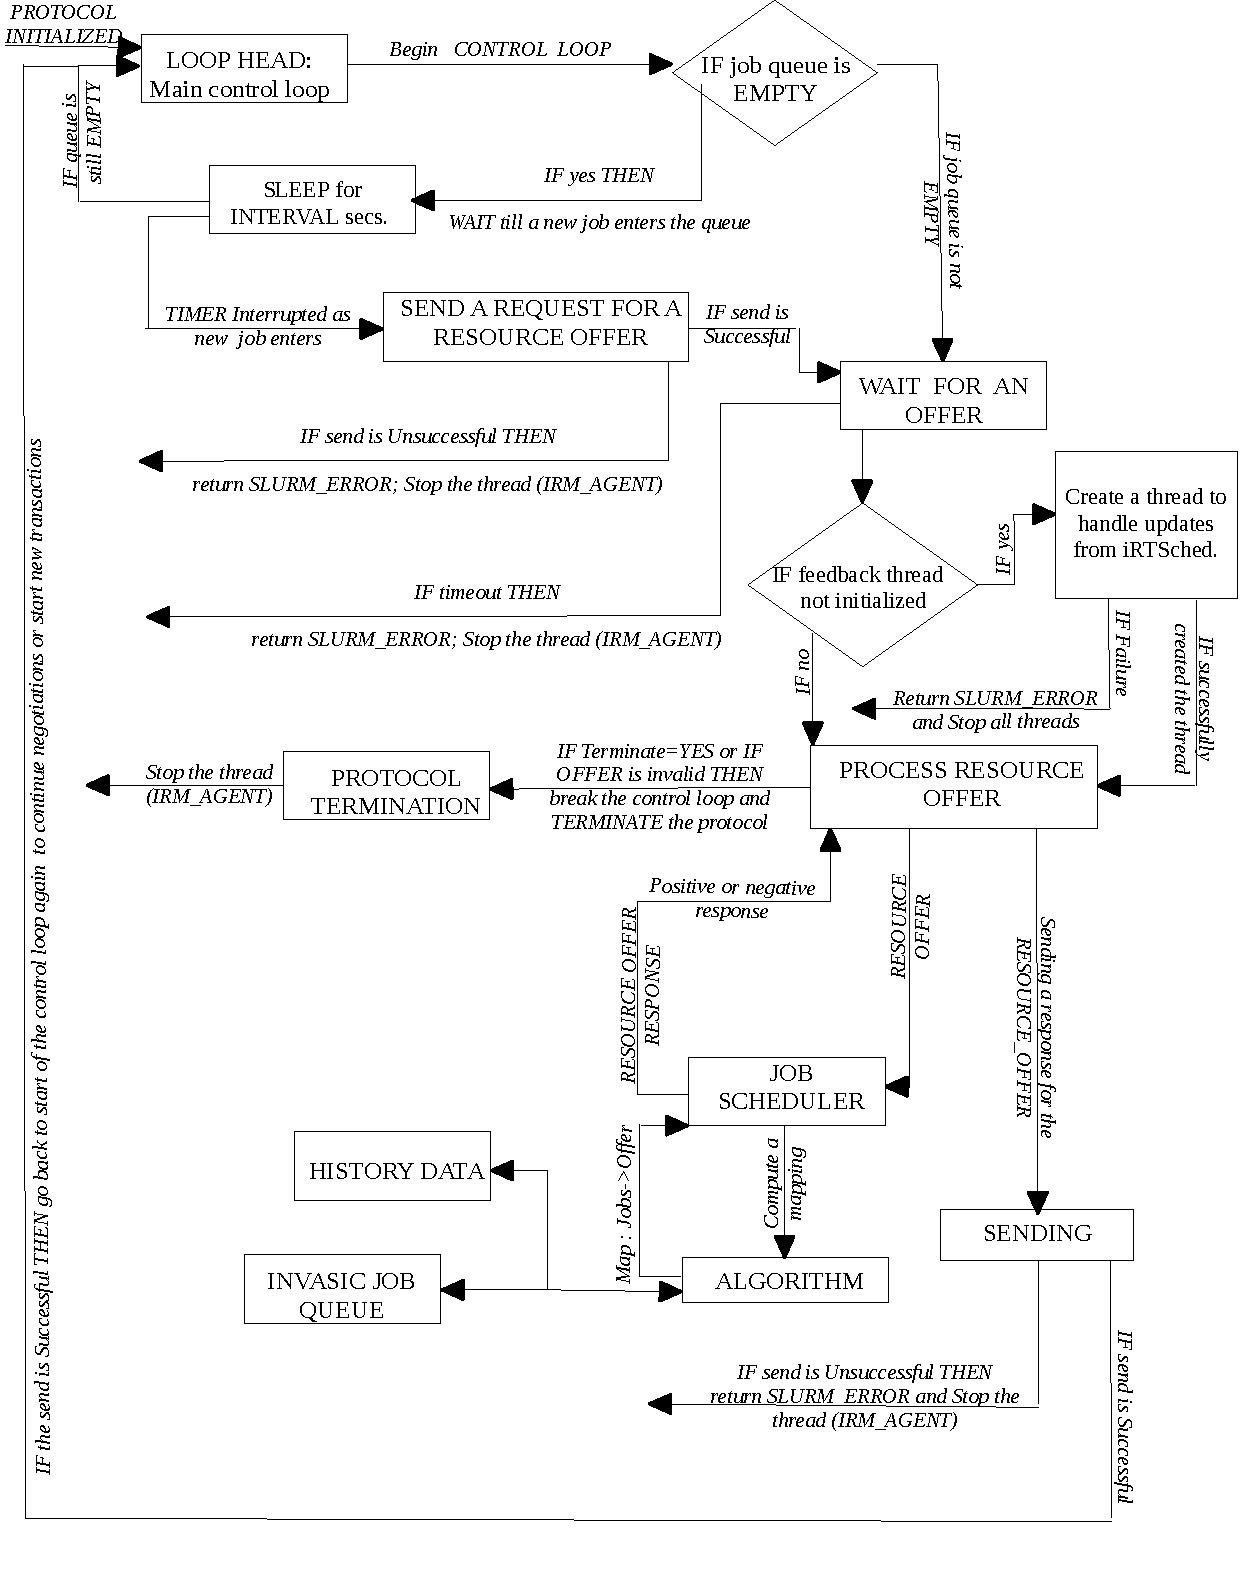
\includegraphics[width=1.0\textwidth, height=195mm]{./figures/iBSched.pdf}
%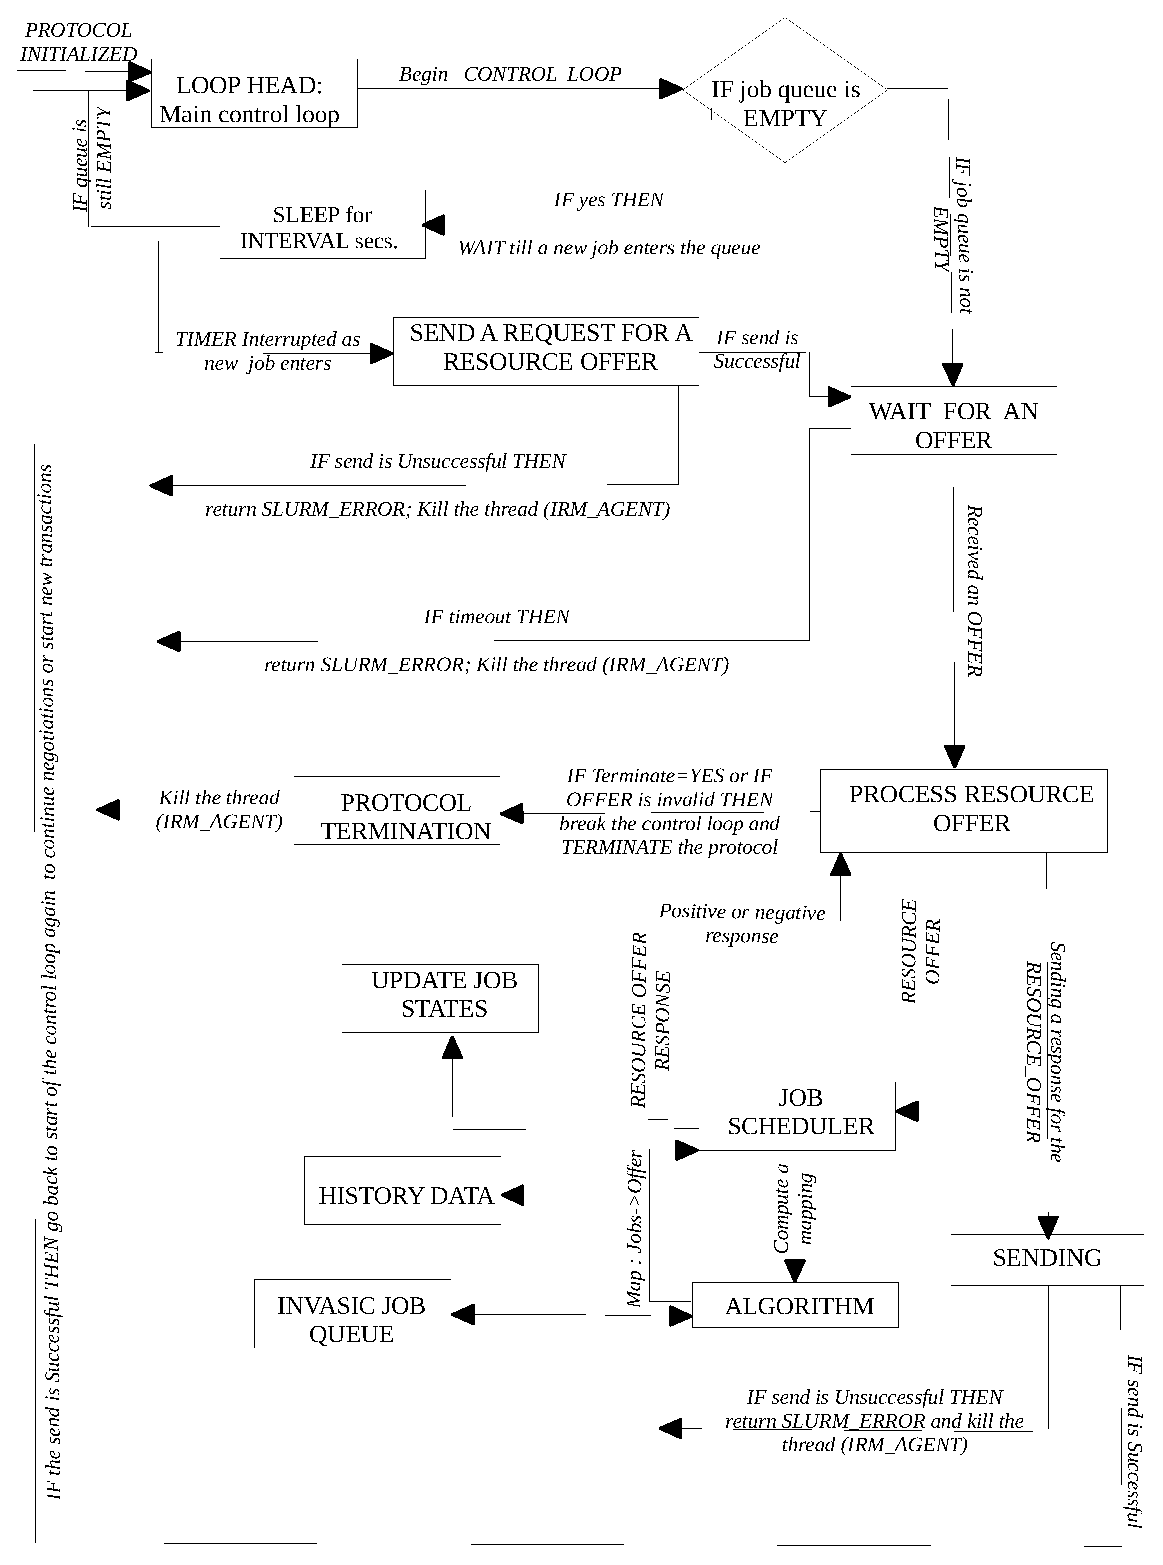
\includegraphics[width=1.0\textwidth, height=180mm]{./figures/Negotiation.eps}
\caption{iBSched}
\label{fig:Neg}
\end{figure}
\noindent
iBSched is a SLURM plugin, hence it is dynamically loaded by the SLURM controller(slurmctld) due to which a plugin initialization happens for iBSched during which a main plugin thread is created. This plugin thread is then responsible to create the main control thread for iBSched. The plugin thread is responsible for starting and shutting down this plugin(in case slurmctld sends a shutdown signal) and other threads it spawned. The main control thread is responsible for shutting down all the slave threads it had spawned. iRTSched also has multithreaded design exactly similat to iBSched except that it is an independent binary and is launched independently but not by any SLURM application.
%\begin{figure}[!htbp]
%\hspace*{0.1in}
%\centering
%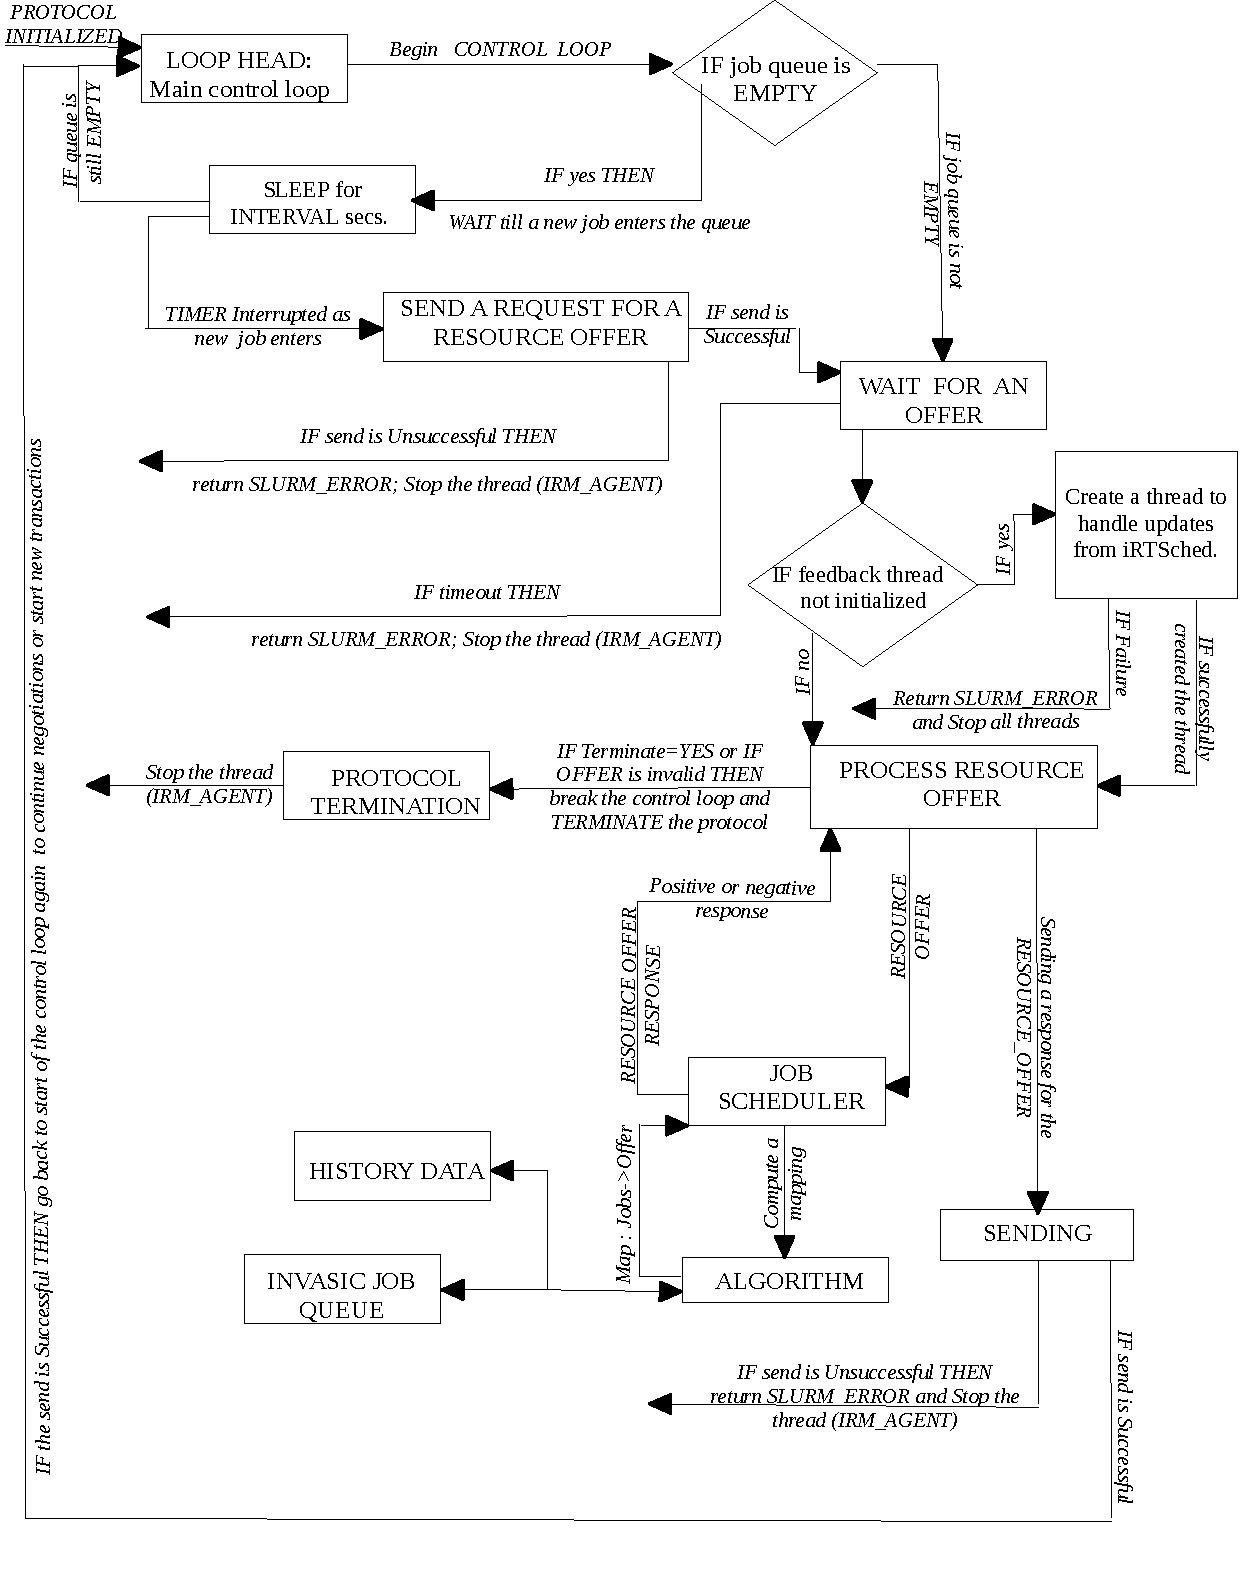
\includegraphics[width=1.0\textwidth, height=195mm]{./figures/iBSched.pdf}
%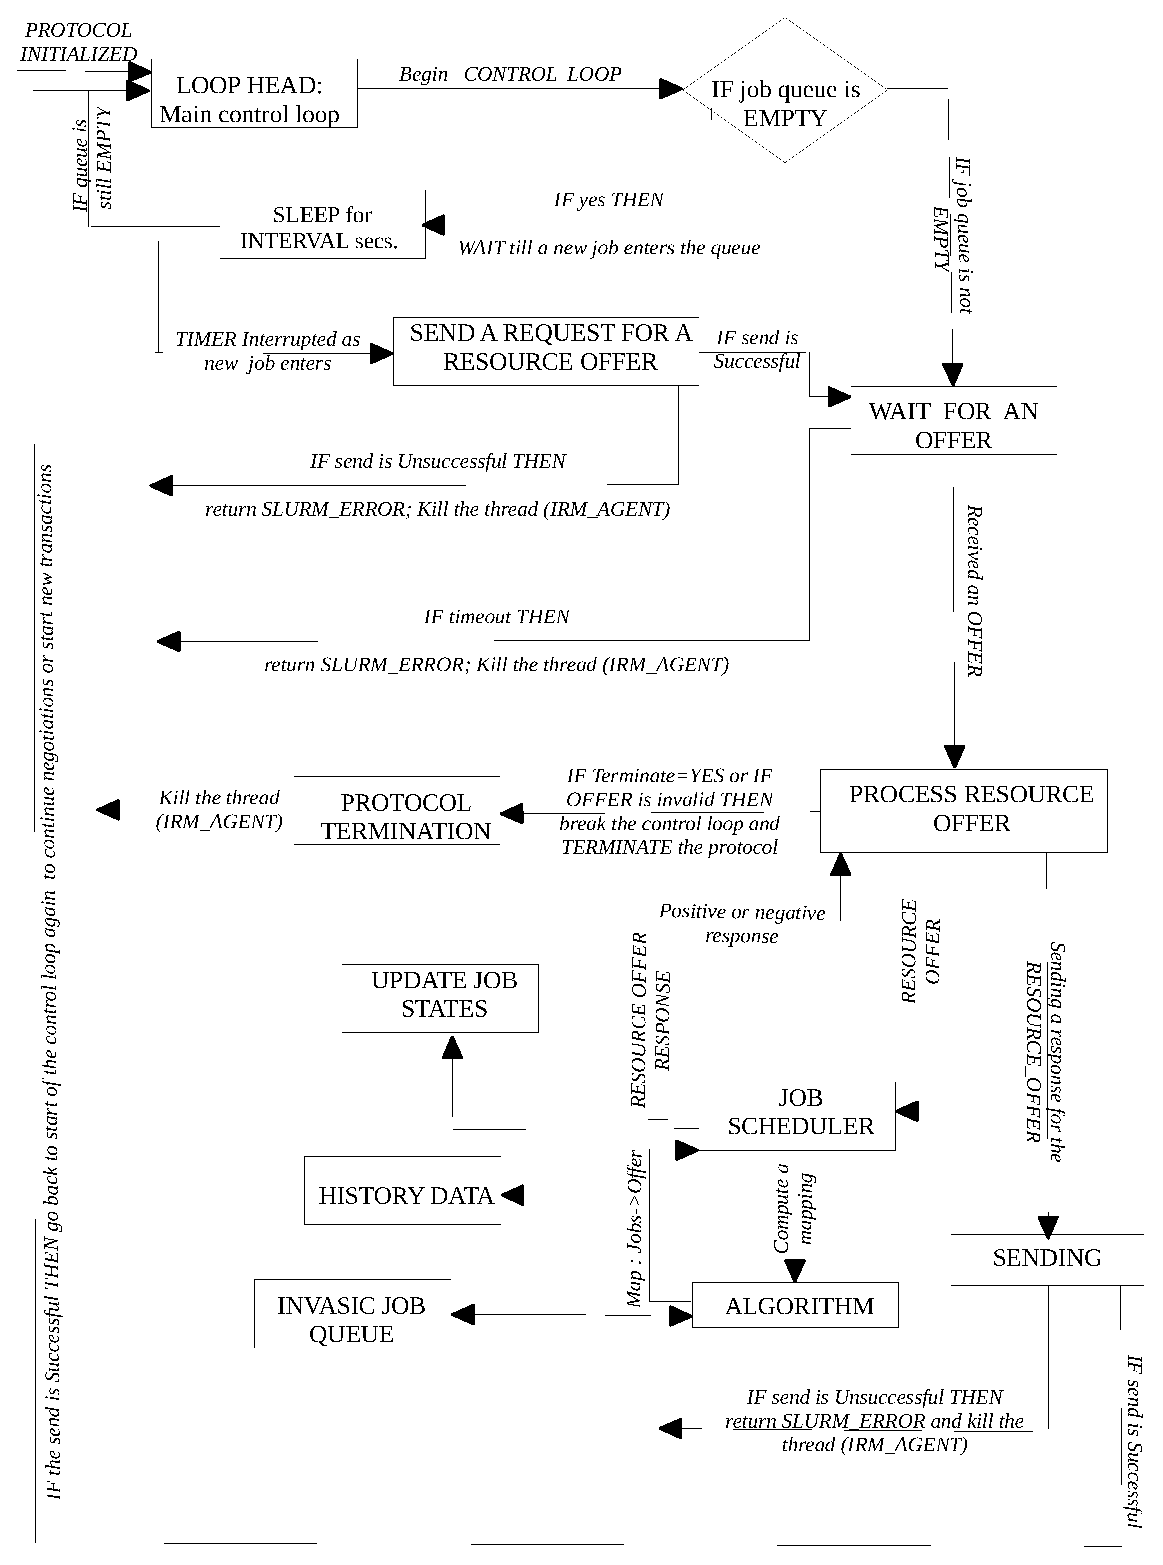
\includegraphics[width=1.0\textwidth, height=180mm]{./figures/Negotiation.eps}
%\caption{iBSched}
%\label{fig:Neg}
%\end{figure}
\begin{figure}[!htbp]
\centering
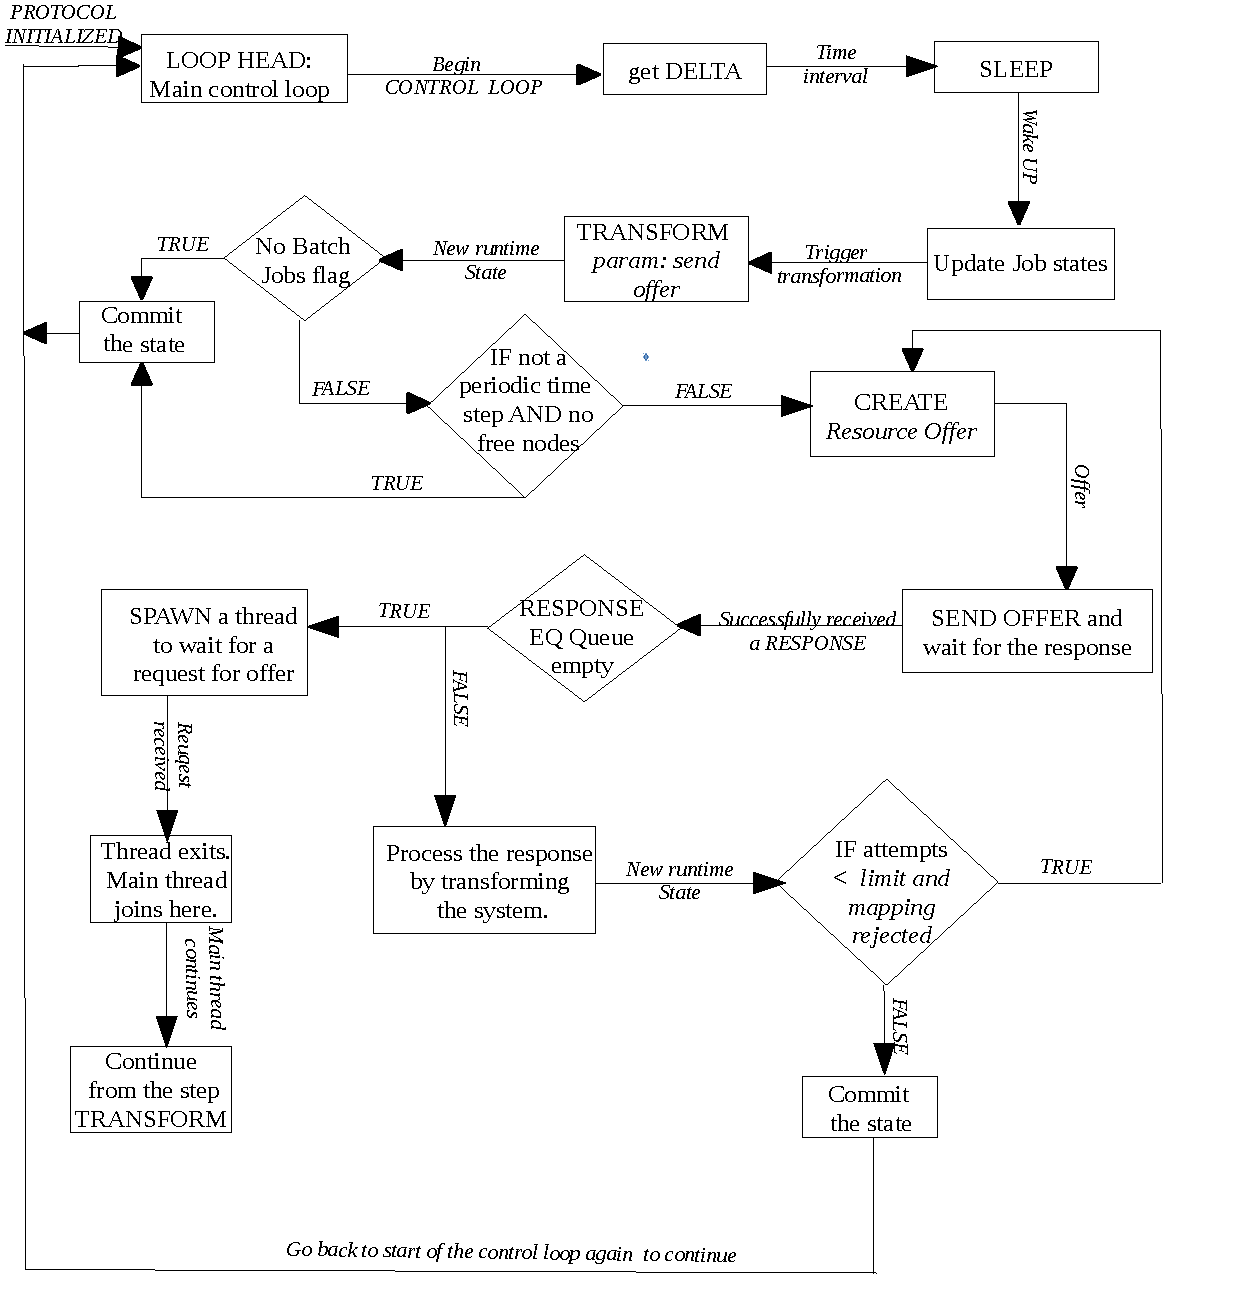
\includegraphics[width=1.0\textwidth, height=160mm]{./figures/iRTSched.pdf}
%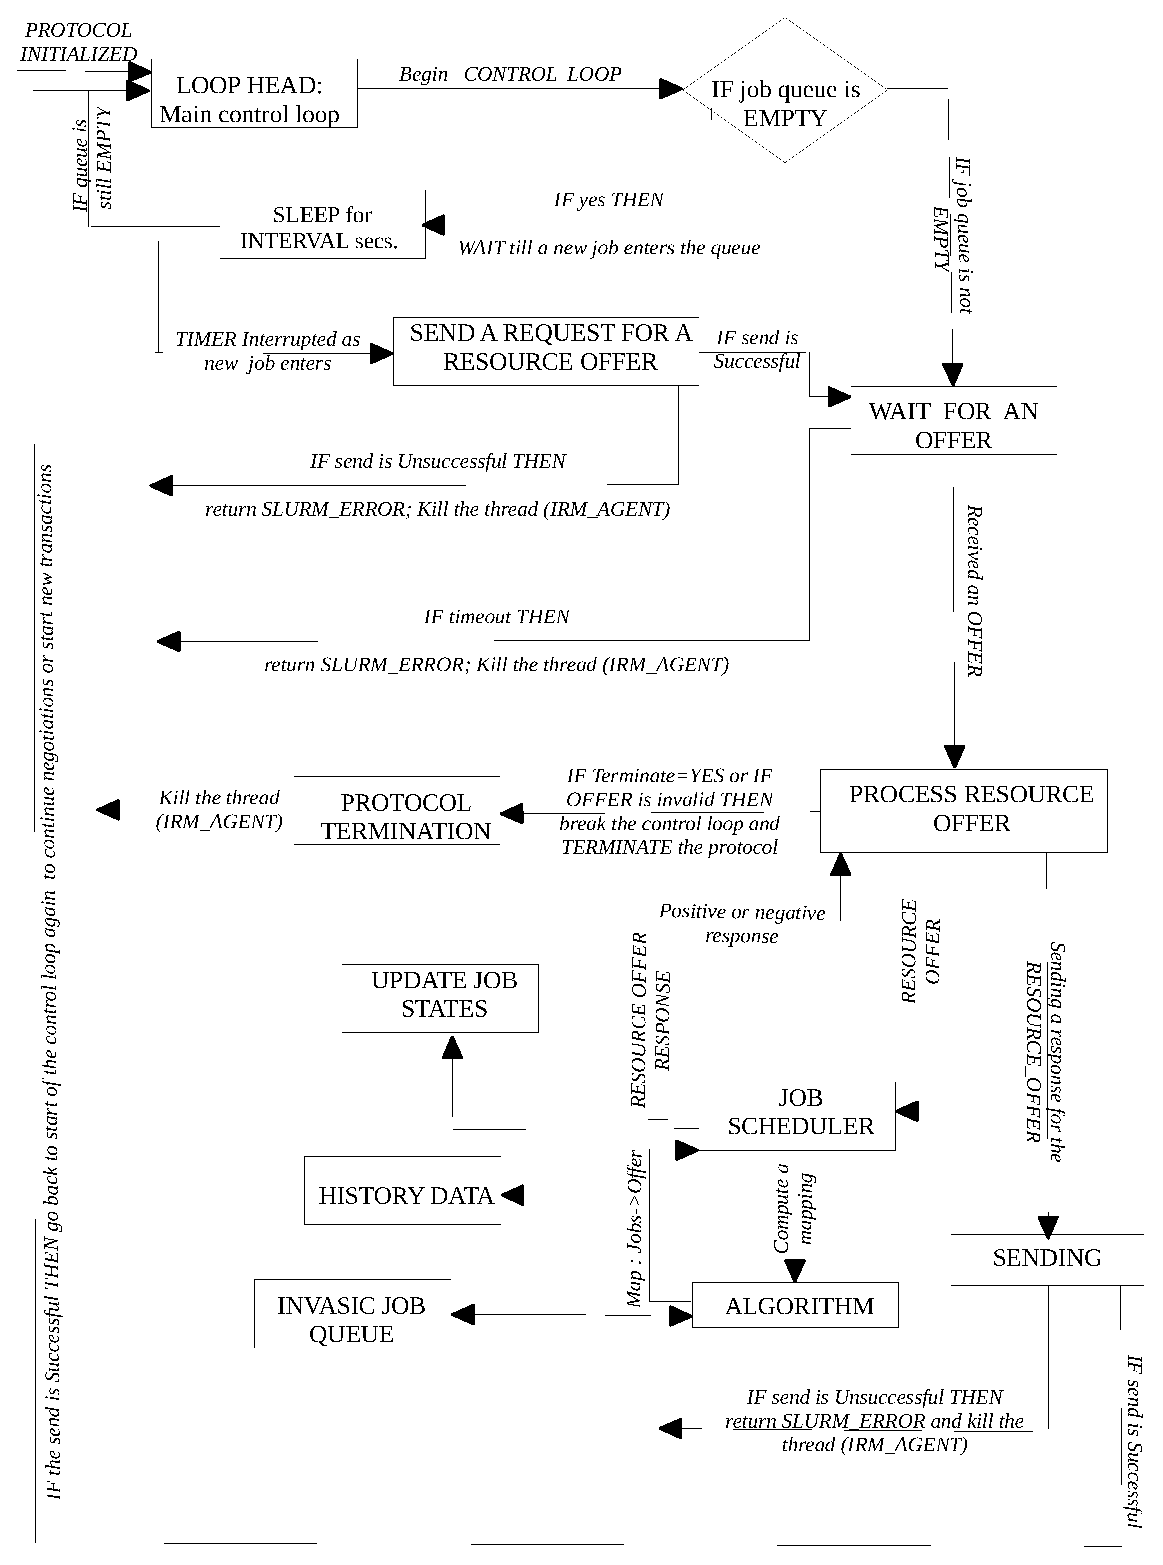
\includegraphics[width=1.0\textwidth, height=180mm]{./figures/Negotiation.eps}
\caption{iRTSched}
\label{fig:Neg1}
\end{figure}
